\chapter{外文资料的调研阅读报告或书面翻译}

\title{Xen 与虚拟化的艺术}

{\heiti 摘要:} 人们设计了无数的系统以通过虚拟化技术分享现代计算机的充足的计算资源。
其中,有的系统需要特制的硬件,或者不能运行日常使用的操作系统;有的为了百分之百的二进制兼容
不得不以性能作为代价;还有的为了性能好牺牲了安全性和功能性。只有很少的一部分提供资源隔离和
性能的保障,大多数只提供“尽力而为”的表现,承担着很高的拒绝服务风险。

在本文中,一个叫做 Xen 的 X86 虚拟化管理程序被提出出来。它使多个常见的操作系统可以以安全、
资源可控而且性能功能都有保障的方式,共享传统的硬件设备。这是通过提供理想化的虚拟机抽象达到的,
常见的操作系统例如 Linux 、 BSD 还有 Windows XP 可以只需很少的努力移植到这个平台。

我们的设计指标允许多达 100 台虚拟机实例在一台物理服务器主机上同时运行。我们采用的虚拟化方法
是非常高效的,例如 Linux 和 Windows XP 的操作系统可以在我们的平台上以极少的性能开销共同
运行——相较于直接运行在物理机上只有百分之个位数的开销。无论在微基准测试,还是在全系统的测试上,
我们的系统都极大地超越了与其竞争的商业和免费的现有解决方案。

\section{引言}

现代的计算机足够强大,可以通过虚拟化技术启动许多小的“虚拟机”,并在每个虚拟机上运行一个独立的
操作系统实例。这导致了虚拟化技术研究兴趣的回潮。在本文中,我们提出了 Xen ,一个高性能、资源
可控的虚拟机管理程序,它可以支持服务器联合、协同托管服务、分布式 web 服务、安全计算平台和
应用程序移动性等多种应用。

成功地将一台主机划分成并行执行的多个操作系统具有以下几个挑战:首先,虚拟机必须保证互相隔离,
它们的执行过程互相影响是不能接受的。尤其是在虚拟机被多个互相不信任的用户共同使用的情况下。
其次,必须支持多种操作系统,才能适应流行的应用程序的多样性。最后,虚拟化带来的开销应该尽可能小。

Xen 可以承载常见的操作系统,尽管需要进行源代码的更改。本文中描述和评估的 Xen 样本支持多个
并行执行的 XenoLinux 客户操作系统实例,每个实例向上对应用程序提供和非虚拟化的 Linux 2.4
完全相同的二进制接口。我们对 Windows XP 的移植虽然是不完整的,但是已经可以运行简单的用户态
应用程序。我们还在移植 NetBSD 操作系统。

Xen 允许用户动态地实例化一个操作系统,使其可以在用户希望的任何地方运行。在 XenoLinux
项目中,我们在互联网提供商和互联网交换机的较为经济的位置上的物理节点上部署了 Xen 系统。
我们在它开启新的虚拟机前进行了准入控制,并且希望每个虚拟机为它所需的资源付出相应的“代价”。
我们会在另外的地方从这个角度讨论我们的想法和实现方法,本文更多地还是关注虚拟机管理程序本身。

在一个共享的物理系统上部署多种应用程序和服务有很多种方法,其中很可能是最简单的一种就是部署
多个主机,每个运行一个标准的如 Linux 或者 Windows 的操作系统,然后用户可以安装文件、
开启程序,应用程序之间的保护机制是由传统的操作系统技术实现的。经验表明,如果这样做,系统
管理工作很快就会变成一项耗时的任务,因为本该互相隔离的应用程序之间复杂的交互配置。

更重要的是,这种系统支持的性能隔离还不够——一个进程的调度优先顺序、内存需求、网络流量还有
磁盘访问会直接影响其它程序的。对于事先规划好的固定的用户群体,这个也许是可以接受的(比如
网格计算或者实验性的 PlanetLab 平台),但是如果资源被过度订阅,或者用户互相协作不愉快,
那么这个模式就不可行。

一个解决方式是翻新操作系统本身对于性能隔离的支持。Resource container 技术、Linux/RK 、
QLinux 和 SILK 或多或少都表现出这个思想。一个主要的困难是保证所有资源占用的帐都记到正确的
那个进程的头上——尤其是考虑到例如缓冲区缓存或者页置换算法导致的应用程序之间复杂的交互。在
操作系统内部这是被称为“QoS crosstalk“的问题。降低复用率可以缓解这个问题,正如 Exokernel
和 Nemesis 操作系统展示的那样。在它们的实现中非刻意的或者不需要的进程间交互被降低到了最低。

我们使用类似的基本方法来创造 Xen ,在 Xen 中物理资源被以整个操作系统的粒度进行复用,
并且能提供它们之间的性能隔离。和进程级的复用不同的是,这种复用允许多个不同的客户操作系统
优雅地共同存在,而不是使用同一个应用层二进制接口。当然,这样的灵活性肯定要付出代价——运行整个
完整的操作系统肯定比运行单个进程更加“重量”,无论是从开机启动来说,还是从资源消耗来讲。

对于我们的目标也就是多达 100 个承载的虚拟机实例,我们相信上述代价是值得的,因为它单个用户
以资源可控制的方式运行未经修改的二进制或者一族二进制程序,例如一个 Apache 服务再加上一个
PostgreSQL 后端)。另外,它还提供了极致的灵活性,因为用户可以精确地恰到好处地创建那个
应用需要的运行环境。麻烦的在多个服务和应用之间的配置协调被避免了(比如说,每个 Windows 实例
可以维护自己独立的注册表)。

本论文的如下部分这样组织:在第二章我们介绍实现虚拟化的具体方法和 Xen 的基本工作原理。
在第三章介绍我们的设计和实现的一些关键细节。在第四章我们使用工业界标准的基准测试程序对在
Xen 上运行的 XenoLinux 内核与在物理机上运行的 Linux 内核、VMWare Workstation 还有
用户态 Linux (UML) 进行比较测试。第五章评价相关工作。第六章介绍后续工作和结论。

\section{Xen: 方法与概述}

在传统的虚拟机管理程序里,虚拟化软件对上层暴露出和下层的硬件完全相同的功能。尽管全虚拟化
有着显而易见的优点,也就是允许未经修改的操作系统在上面运行,但是它有几个缺点。对于流行的
IA-32 / X86 架构来说,更是如此。

对于全虚拟化的支持从来就不是 X86 体系结构的一部分。特定的内核指令必须经过虚拟机管理程序的
处理才能实现正确的虚拟化,但是在不足的权限下运行这些指令会悄无声息地失败,而不是导致易于
处理的陷入。高效率地将 X86 的 MMU 进行虚拟化也是非常困难的。这些问题当然都可以被解决,
只不过需要以增加的复杂度和降低的效率作为代价。VMWare 的 ESX Server 自动地重写一部分客户机
的代码来插入陷入,每当虚拟机管理程序必须介入执行的时候。这个翻译过程必须应用到整个客户机的
操作系统内核上(带来相应的翻译、执行、缓存的开销)因为所有不会带来陷入的特权指令必须被
捕获和处理。ESX Server 还实现了系统数据结构比如页表的一个“影子”版本,并且通过陷入每个
更新操作维护虚拟页表的一致性——这个实现方法对于更新频繁的操作,比如创建一个新的应用程序进程
带来了非常大的开销。

难以忍受 X86 错综复杂的特性,存在其它反对全虚拟化的讨论。特别是有客户虚拟机想要既能看到真实
的硬件资源又能看到虚拟的硬件资源的实际的应用情况,例如既提供实际的时钟又提供虚拟的时钟可以使
客户虚拟机更好地支持时间敏感的任务,使其准确地处理 TCP 超时以及 RTT 估计,又比如暴露出
物理机的实际地址允许客户机通过使用 superpages 和 page coloring 技术获得更好的性能表现。

我们通过提供一个和下层的硬件类似但是又不完全相同的虚拟机抽象来避免全虚拟化的缺陷——这种方法
被称为“半虚拟化”。这种方法会带来更高的性能,尽管需要修改客户机的操作系统。但是请注意,
我们不需要修改应用程序的二进制接口 ABI ,所以上层应用无须做修改。

我们将上述讨论总结为如下几个原则:

\begin{enumerate}
    \item 支持未经修改的应用程序二进制文件至关重要,否则用户就不会迁移到 Xen 。
    因此我们必须将现有的 ABI 的全部结构特性进行虚拟化;
    \item 支持完整的多任务操作系统是重要的,因为这样可以允许复杂的服务设置在单一的客户机
    操作系统实例内被虚拟化;
    \item 在 X86 这种虚拟化不友好的平台上,半虚拟化是必须的,因为通过它可以获得高性能
    和强的资源隔离;
    \item 即便在虚拟化友好的硬件架构上,完全地对客户操作系统隐藏虚拟化的效用也会带来正确性
    与性能的风险。
\end{enumerate}

注意,我们的 X86 半虚拟化抽象和最近的 Denali 项目提出的设计非常不同。Denali 被设计用来
支持数以千计的运行网络服务的虚拟机,它们中大多数都规模不大并且也不流行。形成对比的是,Xen
的设计目标是支持多达 100 个运行行业标准的应用与服务的虚拟机。因为目标非常不同,将 Denali
的设计方法和我们的原理作对比是有益的。

首先,Denali 的目标不在于已有的 ABI ,所以可以从虚拟机接口中忽略一部分结构特性。
举例来说,Denali 并不完全支持 X86 的分段机制,尽管它在 NetBSD 、Linux 和 Windows XP
的 ABI 中广泛使用。

其次,Denali 的实现方法没有解决支持应用程序复用或者一个客户操作系统的不同的地址空间的问题。
应用程序被以类似 Exokernel 中的 libOS 的形式显式地链接向一个 Ilwaco 客户操作系统的实例。
因此,每个虚拟机只能承载一个单用户模式的单应用的未经保护的所谓“操作系统”。形成对比的是,
在 Xen 中,一个虚拟机可以承载一个真正的操作系统,在这个操作系统上又可以复用出成千上万的
未经修改的用户态进程。尽管一个原型虚拟 MMU 被开发出来用于帮助 Denali 达到类似的目标,
但是我们没有看到任何已发表的技术细节或者评估报告。

再次,在 Denali 的架构中虚拟机管理程序通过磁盘输入输出操作所有分页机制。这可能是因为在
虚拟化层缺少内存管理机制。在虚拟机管理程序内部解决分页机制和我们的进行性能隔离的目标向左:
恶意的虚拟机会激励内存抖动,不公平地把别的虚拟机的 CPU 时间和磁盘带宽据为己有。在 Xen 系统中
我们希望每个客户机都有自己的分页机制,使用自己分配到的那一份内存空间和磁盘份额。

最后,Denali 将每台机器的资源的命名空间进行了虚拟化,采用了如果一台虚拟机不能对另一台虚拟机
的资源进行命名那么就无法访问该资源的方式。举例来说,虚拟机们对硬件地址一无所知,它们只知道
Denali 为它们创建的虚拟地址。相反,我们认为虚拟机管理程序内部的安全访问管理对于保护来说
已经足够了,另外,正如上文讨论过的,如果使物理资源被客户操作系统直接访问会带来很激烈的正确性
与性能的争论。

在下面的一节中我们讨论 Xen 的虚拟机抽象,并讨论 Xen 如何通过修改客户操作系统来达到这一点的。
注意,在本文中,我们使用术语“客户操作系统”来指代 Xen 可以承载的操作系统之一,使用“域”来指代
一个运行着某个“客户操作系统”的虚拟机;这个区别好似在传统的系统中程序与进程的概念。我们管 Xen
本身叫做虚拟机管理程序 (hypervisor) 因为它执行的特权级相对于它承载的客户操作系统的内核更高。

\begin{figure}[h]
    \centering
    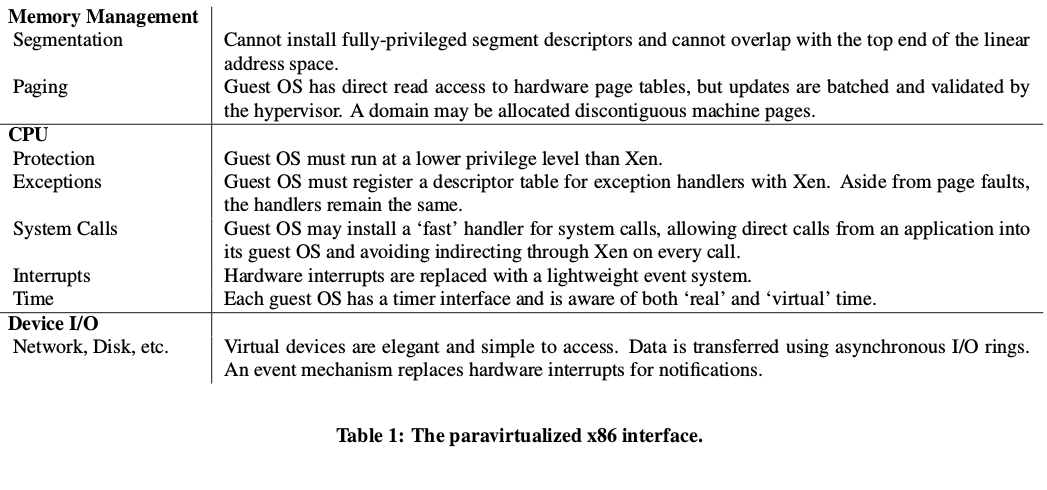
\includegraphics[width=\textwidth]{the-paravirt-x86-interface}
\end{figure}

\subsection{虚拟机接口}

表 1 展示了 X86 半虚拟化接口的一个概览,主要可以划分为三个大块:内存管理、CPU 还有
输入输出设备。在下面的章节我们依次介绍三个子系统,并讨论每个部分是如何在我们的半虚拟化架构中
被表示的。注意,尽管我们的实现中的一部分,比如内存管理,是特定地针对 X86 平台的,许多方面
例如虚拟 CPU 和输入输出设备可以直接应用到别的体系结构上。另外,X86 体系结构代表了它区别于
RISC 体系结构的最坏的一种可能性,比如说,有效地将硬件页表虚拟化比将软件控制的 TLB
虚拟化要更加复杂。

\subsubsection{内存管理}

将内存虚拟化毫无疑问是将体系结构半虚拟化中最困难的部分,无论是从虚拟机管理程序的原理上讲,
还是从每种客户操作系统被移植的工作量上讲。如果体系结构本身提供一个软件管理的 TLB 那么这个
工作就更加容易了,因为这样的结构能简单有效地被虚拟化。TLB 标记是另一种被多数服务器级的 RISC
体系结构支持的有用的功能,比方说 Alpha 、MIPS 还有 SPARC 。将地址空间标志位同每个 TLB
表项联系起来使得虚拟机管理程序与每个客户操作系统有效地在分开的地址空间里共同存在,因为在二者
转换执行的时候就没有必要清空掉整个 TLB 了。

遗憾的是,X86 并没有软件控制的 TLB ,与此相反的是 TLB 缺失被 CPU 本身以遍历整个页表结构
的形式自动处理。因此为了达到最好的性能,所有有效的对于当前的地址空间内的页地址转换都需要在硬件
可访问的页表中存在。另外,因为 TLB 没有标记,地址空间转换通常需要清空整个 TLB 。基于这些限制,
我们作出了两个决定:(1) 客户操作系统负责分配和管理硬件页表,Xen 的介入非常至少来保证安全性
和隔离性;(2) Xen 在每段地址空间的上 64 MB 存在,因此避免进入退出虚拟机管理程序造成的 TLB
清空。

每次一个客户操作系统需要一个新的页表——也许是因为一个新的进程创建了——它从它自己的内存保留
区域内分配并初始化一页并在 Xen 上做登记。此时,操作系统必须放弃对页表所在的内存区域直接写入
的权限,之后所有的更新都需要被 Xen 批准。更新在几个方面被限制,包括只允许操作系统对它拥有的页
进行映射,并且禁用页表的可写入映射。客户操作系统可以通过一次送入一批更新请求的方式来减少进入
虚拟机管理程序的开销。每个地址空间上方 64MB 预留给 Xen ,对于客户操作系统是不可访问或者
重新映射的。这个地址区域不被任何常见的 X86 ABI 使用,所以这个限制不会影响应用程序的兼容性。

分段被用类似的方式进行虚拟化,就是批准对硬件段描述符表的更新。X86 里的段描述符惟独的限制是:
(1) 它们的特权级比 Xen 低;(2) 它们不允许任何对 Xen 预留的地址空间的访问。

\subsubsection{CPU}

对 CPU 进行虚拟化对于客户操作系统来说有几个含义:首先,在客户操作系统下方插入虚拟机管理程序
和传统意义上的“操作系统才是特权最高的”的概念相违背。为了保护虚拟机管理程序免于操作系统的
异常行为(以及域与域之间的隔离),客户操作系统必须进行修改在更低的特权级上运行。

很多的处理器体系结构只提供两个特权级。在这种情况下,客户操作系统会与应用程序一起共享较低的
特权级。客户操作系统通过在与应用程序不同的地址空间里运行而把自己保护起来,通过虚拟机管理程序
设置虚拟的特权级和改换当前地址空间从而间接地与应用程序交替运行。如果处理器的 TLB 支持地址空间
标记,那么代价昂贵的 TLB 清空就可以被避免了。

高效地将特权级进行虚拟化在 X86 上是可行的,因为它在硬件层面支持四个不同的特权级。X86 的特权级
一般被称为 rings ,从 0 到 3 。操作系统的代码通常在 ring 0 执行,因为其它的 ring 都不能
执行特权指令,而 ring 3 一般被应用程序的代码使用。据我们所知,ring 1 和 ring 2 自从 OS/2
就没有被任何著名的 X86 操作系统使用过。任何符合这个特点的操作系统都可以被移植到 Xen 上通过
修改以在 ring 1 里运行。这可以防止客户操作系统直接运行特权指令,并且可以和 ring 3 上运行的
应用程序隔离开来。

特权指令通过在 Xen 内部批准和执行来半虚拟化。这些适用于类似创建一个新的页表或者在空闲时放弃
CPU 资源等操作。任何客户操作系统的直接执行特权指令的尝试都会被处理器本身拒绝掉,或者是静默地
或者产生一个错误,因为只有 Xen 本身才能在一个权限足够的层级运行。

异常,包括内存异常和软件的陷入,在 X86 上的虚拟化都十分直接。描述每种异常的处理程序的表在
Xen 上登记待批准。这些在表中声明的处理程序基本上和对于真实 X86 硬件的相同。这是可行的,
因为在我们的半虚拟化架构中异常的栈帧没有被修改。唯一的修改是对于缺页异常的处理程序,它通常是
从特权寄存器 CR2 中读取缺页的地址,但是因为这是不可能的,我们把它写在了一个扩展的栈帧里。
每当一个异常发生在在 ring 0 外执行,Xen 的处理程序创建客户操作系统上异常栈帧的一个拷贝,
然后把控制权交给注册的处理程序。

通常,只有两类异常的发生会频繁到影响系统性能的地步:系统调用(它们通常是通过软件异常实现的)
还有缺页异常。我们通过允许每个客户机操作系统注册一个“快的”异常处理程序,它可以被处理器直接访问
而不是间接通过 ring 0,来提高系统调用的性能。这个处理程序在被写到硬件异常表中之前就被有效化了。
遗憾的是,不能对缺页处理程序使用相同的技术,因为只有 ring 0 里执行的代码才能访问 CR2 里
存储的缺页地址,缺页异常必须通过 Xen 被传送一次,使得寄存器的值能从 ring 1 中访问。

安全性是由直到异常处理程序被传给 Xen 才被有效化而保证的。唯一需要的检查是处理程序的代码段
不会提出去 ring 0 执行。因为没有客户操作系统能创建类似的段,它有能力比较那个段选择子与 Xen
预留的几个静态的值之间的大小关系。除此之外,其它的一些处理程序的问题会在异常的传输过程中被解决
——举例来说,如果处理程序的代码段不存在或是处理程序没有被进行内存分页,那么当 Xen 执行 iret
指令返回处理程序的时候,相应的异常就会被处理。Xen 通过检查异常程序的计数器来检测“双误”
(double faults) ,如果地址处于异常虚拟化的代码处,那么触犯的客户操作系统会被终止。

请注意,即使对于直接的系统调用处理程序,惰性检查也是安全的,因为访问异常只有当 CPU 尝试直接
跳转到客户操作系统的处理程序时才会发生。在这种情况下,异常的地址是在 Xen 之外的,因为 Xen
永远也不会调用客户操作系统的系统调用,所以异常被虚拟化的方法是正常的。如果异常在传导过程中
导致了双误,那么客户操作系统会被以如上方式终止。

\subsubsection{设备 I/O}

和全虚拟化环境中模拟现实存在的硬件设备不同的是,Xen 暴露出的是清晰而简单的设备抽象。
这就允许我们设计出一个既高效又满足对于保护和隔离的需要的接口。为此,I/O 数据通过 Xen
在各个域之间传递,使用的是共享内存的、异步的缓冲区描述符的环 (buffer-descriptor rings) 。
这就提供了一个高效的在系统中垂直传递缓冲区信息的通讯机制,Xen 可以借此实现高效率的有效性检查,
比如检查包含在域的保留内存内的缓冲区)。

与硬件中断相似,Xen 支持一种轻量的传送机制,它被用来向一个域发送异步的通知。这些通知是通过
更新待完成的事件类型的一个位映射实现的,也可以选择使用调用由客户操作系统指明的事件处理程序。
这些事件的回调可能会因为客户操作系统的决策而被暂缓——比如说为了减少因为频繁的唤醒导致的额外的开销。

\subsection{向 Xen 移植操作系统的开销}

\begin{figure}[h]
    \centering
    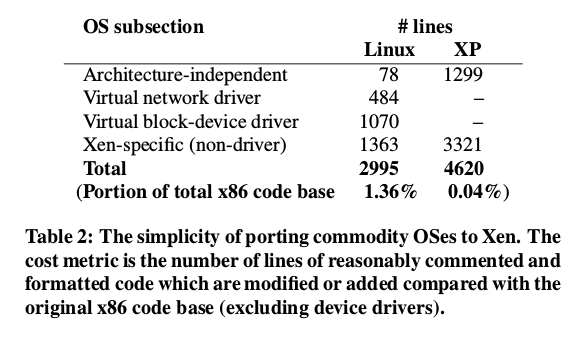
\includegraphics[width=0.8\textwidth]{xen-porting-simplicity}
\end{figure}

表 2 通过代码行数展示了向 Xen 的半虚拟化环境移植常见操作系统的代价。注意我们的 NetBSD 移植
尚处在非常初始的阶段,所以没把它的数据加入表格。Windows XP 的移植处于更高级的阶段,但是也尚
未完工,它可以从 ramdisk 中执行一些用户态的程序,但是全部虚拟 I/O 都还不好使。正因如此,所有
XP 的虚拟设备驱动的数据都没有在图表中出现。但是对于 Linux 来说,我们认为这些驱动都是短小精悍
的,因为 Xen 提供了理想化的硬件抽象。

Windows 令人惊讶地需要极大量对于机器无关代码部分的修改,因为它访问页表项 PTE 使用了很多种
不同的数据结构与联合。每种页表的访问都需要被单独修改,尽管一部分可以通过脚本来自动化。恰恰相反
的是 Linux 需要的对于内存系统的修改相对来说非常少,因为它使用预处理的宏来访问 PTE ——往预处理
宏内加入半虚拟化需要的翻译和虚拟机管理程序的调用就要方便多了。

在两种操作系统中,体系结构相关的部分都是我们从 X86 移植到半虚拟化要显著改写的。这包括改写
使用了特权指令的例程,还有移除大量的底层的系统初始化代码。再一次,Windows XP 需要的工作量更大,
主要是因为遗留的 16 位模拟层的存在以及需要一个不同的启动-加载机制。主要到在 Windows XP 中
X86 特有的代码比 Linux 里的要显著地更多,所以更大的移植的工作量是可以预见到的。

\subsection{控制与管理}

Xen 的设计与实现从始至终的一个目标就是将策略 (policy) 与机理 (mechanism) 尽可能地分离开。
尽管虚拟机管理程序必须涉及进数据路径的方面,比如在域和域之间切换 CPU 占用,在传输之前过滤
网络的包,或者是在读取数据块的时候保障访问权限控制,它没有必要涉及进更高层的事情,比如 CPU
是如何共享的,或者每个域可能会传输怎样的数据包。

这导致了一个虚拟机管理程序本身仅仅提供基本的控制操作的架构。这些操作通过能被从授权的域访问的
接口导出到上层。潜在复杂的策略,比如准入控制,最好是由在客户操作系统中运行的管理软件来完成,
而不是在特权的虚拟机管理程序的代码里做。

\begin{figure}[h]
    \centering
    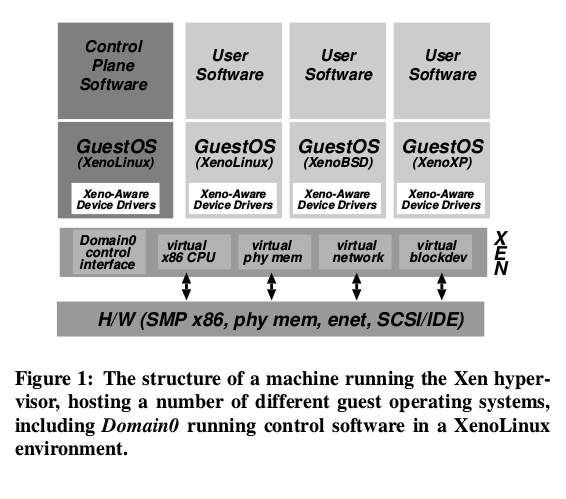
\includegraphics[width=0.7\textwidth]{xen-arch-orig}
\end{figure}

整体上的系统架构如图 1 所示。注意一个域在启动时被创建,允许使用控制接口。最初的域,叫做
Domain0 ,负责运行应用层的管理软件。控制接口提供了创建和终止其它域的能力,并且能控制他们关联
的调度的参数、物理内存分配还有物理机的磁盘和网络设备配给的访问权限。

除了处理器和内存资源之外,控制接口还支持虚拟网络接口 (VIF) 和块设备 (VBD) 的创建与删除。
这些虚拟的 I/O 设备具有关联的访问控制信息,决定了哪个域能访问它们,并且受到哪些限制。举例来说,
一个只读的 VBD 可能被创建,或者一个 VIF 可能会通过过滤 IP 包来防止源地址伪造。

控制接口与当前系统状态的统计信息,导出到一个在 Domain0 中运行的应用层管理软件套件中。这个对于
管理工具的补足使得方面地管理整个服务器成为可能:当前的工具可以创建或者销毁域、设置网络过滤器和
例程的规则、在数据包和数据流的粒度监控每一个域的网络状态、创建和删除虚拟网络接口和虚拟的块设备。
我们预期对高层的工具的开发会使得管理策略应用的自动化更进一步。

\section{设计的细节}

在本章中我们介绍组成基于 Xen 的服务器的几个主要的子系统。为了展示得清楚,在每个情况里我们既
展示 Xen 的也展示客户操作系统的功能。目前对于客户操作系统的讨论集中在 XenoLinux 身上,因为
它是当前最为成熟的。尽管如此,我们接下来的对 Windows XP 以及 NetBSD 的移植工作给了我们 Xen
是客户操作系统无关的信心。

\subsection{控制的传输——Hypercall 与事件}

Xen 与它上面的域存在两个控制交互的机制,同步的从域到 Xen 的调用可以通过 hypercall 实现,
而从 Xen 到域的通知 (notification) 则是使用一个异步的事件 (event) 机制实现。

Hypercall 的接口使得域能够产生一个进入到虚拟机管理程序的同步的软件陷入以进行特权操作,类似于
传统的操作系统里的系统调用的作用。一个 hypercall 的实例应用是要求一系列页表的更新,其中 Xen
批准和应用了一系列更新,在完成之后返回调用的域继续执行。

从 Xen 到域的通讯是由异步的事件机制实现的,它取代了传统的设备终端的传送机制,允许重要事件使用
轻量的通知 (notification),例如终止一个域的请求。类似于传统的 Unix 的信号 (signal) 机制,
只有少数几个事件,每个标志一种特殊类型的出现。举例来说,事件被用来显示网络传来了新数据,或者
一个虚拟磁盘请求完成了。

暂缓的事件存储在每个域都有的一个位映射区域内,在唤起由客户操作系统指明的事件回调处理程序之前
由 Xen 进行更新。回调处理程序负责重置暂缓事件的集合,还负责以正确的方式响应通知
(notification) 。域可以通过设置 Xen 可读的软件标记来显式地推迟事件的处理,这与在真实的
处理器上关闭中断的办法是相似的。

\subsection{数据的传输——I/O 环 (rings)}

虚拟机管理程序的存在意味着在客户操作系统与 I/O 设备之间存在着额外的防护,所以数据传输机制
能够保障数据在系统之中垂直以很小的开销传输就至关重要。

我们的 I/O 传输机制是由两个关键因素决定的——资源管理和事件通知。对于资源的可描述性,我们尝试
最小化分离当中断从设备被接受到时候去向一个特定的域的数据所需的工作——管理缓冲区的开销直到计算
任务被分配给恰当的域的时候才会产生。类似的,设备 I/O 占用的内存是每当防止共享的缓冲区的内在
串扰是可行的的时候,从相关的域提供出来的。I/O 缓冲区在数据传输的时候通过与 Xen 绑定下层的
页帧保护起来。

\begin{figure}[h]
    \centering
    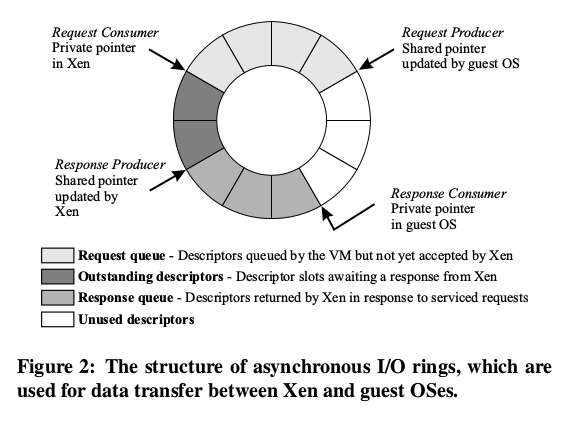
\includegraphics[width=0.7\textwidth]{io-rings}
\end{figure}

图 2 展示了我们的 I/O 描述符的环的结构。一个“环”就是一个由被域分配的描述符组成的环形队列,
它从 Xen 内部是可以访问的。这些描述符并不直接包含 I/O 数据,相反,I/O 数据缓冲区是由客户
操作系统在外面分配并间接被 I/O 描述符引用的。对于每一环的访问是基于两对生产者-消费者指针的:
域在一个环上放置请求,将请求生产者指针加一,然后 Xen 将请求取出进行处理,将一个关联的请求
消费者指针加一。请求的回复也以类似的方式放置回环上,保存成以 Xen 作为生产者、以客户操作系统
作为消费者的模式。请求不需要被顺序地处理,因为客户操作系统将每个请求关联一个唯一的标识符,
这也就导致了关联过的回复。这使得 Xen 因为调度或者优先级的考虑清楚地重排 I/O 操作成为可能。

这个结构足矣支持多个不同的设备范式。举例来说,一系列请求可以为网络包接收提供缓冲区,后续的回复
标志着数据包进入这些缓冲区。处理磁盘请求时重排序是有用的,因为它允许请求在 Xen 内部为了高效率
而进行调度,与外部的缓冲区一起使用描述符使得实现零拷贝 (zero-copy) 传输变容易了。

我们将请求与回复的产生与其它部分的通知解除组对:在请求的情况下,一个域可能会在唤起一个通知
Xen 的 hypercall 之前入队许多项;在回复的情况下,一个域可以通过指定一个回复数的阈值来推迟
通知事件的发送。这使得每个域可以在延迟与吞吐率之间做折衷,这和 ArseNIC 千兆以太网接口中的
flow-aware 中断分配是类似的。

\subsection{子系统虚拟化}

上面描述的控制和数据传输的机制在我们的虚拟化平台的不同子系统中都有应用。在下文中,我们讨论
虚拟化对于 CPU 、时钟、内存、网络和磁盘分别是如何实现的。

\subsubsection{CPU 调度}

Xen 当前使用 BVT (Borrowed Virtual Time) 算法来实现不同域之间的调度。我们选择这个算法
是因为它需要的工作量比较少,另外有一个域接收事件唤醒时候的低延迟的特殊机制。对于最小化在设计
为以适时的方式运行的操作系统子系统上虚拟化的影响来说,快速的分配 (dispatch) 尤为重要。举例
来说,TCP 依赖及时的确认 (acknowledgement) 来正确估计网络来回的时间。BVT 使用虚拟时间扭曲
(virtual-time warping) 提供了低延迟的分配,这是一种临时破坏“理想地”公平的分配方式来偏向
于最近唤醒的域的分配机制。然而别的调度算法也可以通过我们的调度器抽象简单地实现。每一域的调度
参数可以通过运行在 Domain0 里的管理程序来调节。

\subsubsection{时间与时钟}

Xen 为客户操作系统提供了真实时间、虚拟时间、挂钟时间 (wall-clock time) 的概念。真实时间
表示成机器启动后过去的纳秒数量,以进程的循环计数器的精度被维护,而且可以频繁地与外部时间源进行
锁定,例如通过 NTP 。一个域的虚拟时间只有当它在执行的时候才会前进,这通常是用于客户操作系统的
调度器保证它的时间片能被应用进程正确地共享的。最后,挂钟时间定义为当前的真实时间加上的一个
偏置量。这保证了挂钟时间能在不影响真实时间的前进的情况下被调节。

每一个客户操作系统可以编程一对闹钟计时器 (alarm timer) ,一个用于真实时间,一个用于虚拟时间。
客户操作系统应该维护内部的计时器队列并且使用 Xen 提供的闹钟计时器来触发最早的超时。超时用
Xen 的事件机制进行传递。

\subsubsection{虚拟地址转换}

和其它子系统一样, Xen 试图将内存访问以尽可能小的开销进行虚拟化。正如在 2.1.1 小节讨论的,
这个目标被 X86 架构的硬件页表的应用变得更加复杂了。VMWare 采取的方式是提供给每个客户操作系统
一个虚拟的页表,而且是 MMU 不可见的。虚拟机管理程序负责陷入访问虚拟页表,批准更新,并在虚拟
页表和 MMU 可见的“影子”页表之间不断传递更改。这极大地增加了某些客户操作系统操作的开销,
比如创建虚拟地址空间,并且要对硬件更新“访问”和“修改”位进行显式的传导。

尽管全虚拟化强迫必须使用影子页表来提供连续物理地址的“幻觉”,Xen 并不是这样受限的。其实 Xen
只需要参与页表的更新操作就可以了,以避免客户操作系统作出不可接受的改动。因此我们就可以避免使用
“影子页表”带来的额外的复杂性和开销——Xen 的方法是将客户操作系统的页表直接注册到 MMU ,并且把
客户操作系统的权限限制为只读 (read-only) 。页表的更新是通过 hypercall 传递给 Xen 的,
为了保障安全性,请求在应用之前必须先经过批准。

为了实现批准的过程我们将每个机器页帧和一个类型与引用计数关联起来。一个帧在每一个时间节点上只能
是下述的几个互斥的类型其一:页目录 (PD) 、页表 (PT) 、本地描述符表 (LDT) 、全局描述符表
 (GDT) 或者可写 (RW) 。注意到一个客户操作系统总是为自己拥有的页帧创建可读的映射,无论它们
当前的类型是哪一个。一帧直到它的引用计数减到 0 才能被安全地重新分配任务 (retask) 。这个
机制用来维护安全所需要的不变性,比方说,一个域不能对页表的任何部分做可写的映射,因为这要求
相关的那一帧同时为 PT 和 RW 类型。

这个类型系统还被用来跟踪哪一帧被批准在页表中使用。客户操作系统将一帧分配给页表使用的时刻指示
出来——这就需要 Xen 批准一帧中的每个项目,在那以后它的类型被以恰当的方式绑定到 PD 或者 PT 上,
直到客户操作系统接下来发出解绑的请求。这对于当改换页表基地址的时候特别有用,因为它消除了在每次
上下文切换的时候批准新页表的需求。注意一帧不能被重新分配任务 (retask) 直到它既被解绑而且
它的引用计数减少到 0 ,这就阻止了客户操作系统使用解绑请求来绕过引用计数机制。

为了尽量减小 hypercall 的数量,客户操作系统可以在使用单一的 hypercall 应用一系列更新之前,
先在本地维护一个这些更新构成的队列——这在创建新的地址空间的时候大有裨益。但是我们必须保证更新
提交得足够及时来保障正确性。幸运的是,客户操作系统通常会在第一次使用新的映射之前进行一次 TLB
清空操作,这就保证了任何缓存的地址转换都被无效化了。因此,在 TLB 清空之前立即提交缓存的更新
操作通常能够满足正确性要求。尽管如此,有的操作系统在它确定 TLB 里没储存过时条目的时候省略了
清空操作。在这种情况下,使用新的地址映射的第一次请求可能会导致一个页不存在的异常。因此客户
操作系统的异常处理程序必须检查未完成的更新,如果有,那么它们就要被清空,然后导致异常的指令
要重新执行。

\subsubsection{物理内存}

最初的为每个域进行的内存分配,或者称为“预留”,是在域的创建时完成的,内存因此在域和域之间
静态地隔离开,保证了强的隔离性。最大的预留空间必须被声明:如果一个域内部的内存压力上升了,
它可以从 Xen 中声明出更多的内存分页,直到这个预留上限为止。相反,如果一个域想要节省资源,
比如说为了减少不必要的开销,它可以通过将分页释放回 Xen 的方式减少内存占用。

XenoLinux 实现了一个“气球驱动”,它通过在 Xen 和 XenoLinux 的页分配器之间来回传递分页
来调节域的内存占用。尽管我们可以直接修改 Linux 的内存管理例程,“气球驱动”使用现存的操作系统
的功能来实现内存的调节,因此减少了 Linux 移植的难度。尽管如此,半虚拟化可以被用来扩大内存驱动
的功能,举例来说,客户操作系统内存不足的处理机制可以被修改来自动通过从 Xen 要求更多的分页
来缓解内存压力。

大多数操作系统假设内存由至多几个大的相邻的分区组成。因为 Xen 并不保证分配内存相邻的区域,
所以客户操作系统通常自己创造一个连续物理内存的“幻觉”,尽管它们下层的硬件内存的分配是稀疏的。
从物理内存到硬件内存的映射是完全由客户操作系统来负责的,它可以直接维护一个由物理页帧号编号
的数组。Xen 通过提供一个由各个域共享可读的转换数组来支持高效的硬件到物理地址转换——这个数组
的更新必须经过 Xen 批准来确保操作系统拥有和自己相关的硬件页帧。

注意到尽管客户操作系统选择在大多数情况下无视硬件地址,它必须在访问页表的时候使用这个地址转换表,
因为这个过程必须使用硬件地址)。硬件地址也会被暴露给操作系统有限的几个内存管理系统来优化内存
访问。举例来说,一个客户操作系统分配特殊的硬件页以优化一个物理标号的缓存中的放置情况,或是使用
超页 (superpage) 映射自然对齐的连续硬件内存的分块。

\subsubsection{网络}

Xen 提供了虚拟防火墙-路由 (VFR) 的抽象,每个域有一个或者多个虚拟网络接口 (VIF) 逻辑地和
VFR 相连。VIF 看上去和现代的网络接口卡有相似之处:有两个缓冲区描述符的 I/O 环,一个用来传输
一个用来接收。每个方向还有一个关联的规则列表——如果模式匹配了,那么相应的动作会被执行。

Domain0 负责插入删除规则。在典型的状况里,规则是用来防止 IP 地址欺骗的,并且能确保基于目的
IP 地址和端口的正确的分离。规则还可以和 VFR 上的硬件接口关联起来。具体来讲,我们可以设置规则
进行实现传统的防火墙功能,比如说防止输入到非安全端口的网络连接。

要传输一个包客户操作系统只要向传输环中入队一个缓冲区描述符就可以了。Xen 会复制这个描述符,
而且为了保障安全,还要拷贝包头并且执行过滤规则。包的负载并不会被复制,因为我们使用分散-集中
(scatter-gather) DMA ,但是请注意,相关的页帧必须在传输完毕之后被绑定。为了保证公平性,
Xen 实现了一个简单地 Round-robin 包调度器。

为了有效的实现包接收,我们要求客户操作系统使用一个页帧来换取它收到的一个数据包,这就避免了 Xen
和客户操作系统之间的包的复制拷贝,尽管它需要页对齐的接收缓冲区在网络接口层被入队。当一个包
接收到,Xen 立即检查接收规则的集合,来决定目标的 VIF 并且在相关的接收环上将包缓冲区交换一个
页帧。如果没有可用帧,那么这个包就被舍弃掉。

\subsubsection{磁盘}

只有 Domain0 具有不用检查直接访问物理磁盘的能力。其它的域通过虚拟块设备 (VBD) 的抽象访问
非易失性存储设备,这个虚拟设备是由 Domain0 里运行的管理软件创建和配置的。允许 Domain0 管理
VBD 使得 Xen 内部的机制保持简单,而且避免了 Exokernel 使用的 UDF 方案那样的错综复杂的
解决方式。

一个 VBD 将关联的所有者和访问控制信息组织成了一个列表,它可以被 I/O 环机制访问。一个典型的客户
操作系统磁盘调度算法将请求在入队进环之前进行重排序以试图减少响应时间,并且应用区分的服务,
比如说,它可以选择以推测的预取请求作为代价来激进地调度同步的元数据请求。但是因为 Xen 对于实际的
磁盘布局有更深入的了解,我们也支持在 Xen 内部进行重排,这样回复就会被乱序返回。一个 VBD 设备
因此对于客户操作系统看上去有点像 SCSI 磁盘。

对于每个 VBD 虚拟机管理程序都维护一个转换表,它的条目是通过 Domain0 的特权控制接口来创建和
管理的。当接收到一个磁盘请求,Xen 检查 VBD 的标识符和偏置来生成相关的扇区地址和物理设备。
权限检查也在这一步进行。令拷贝的数据传输使用 DMA 在请求的域上的磁盘和绑定的内存页之间进行。

Xen 的服务使用 round-robin 的方式批量处理从相互竞争的域来的请求,在到达磁盘硬件之前还要再
经过一个标准的电梯调度器。当需要维护高级别的语义的时候域可以显式地向下传递重排序的壁垒,比如说
使用预写入的日志时。低级别的调度给予了非常好的吞吐率,请求的批处理保证了相对公平的访问。未来的
工作会考察提供更可预测的隔离和区分的服务,可能会使用现有的技术与调度器。

\subsection{创建新的域}

为了新的域创建初始的客户操作系统结构的任务基本上是靠使用特权控制接口访问新域的内存并通知 Xen
初始的寄存器状态的 Domain0 。这个方式相比于完全靠 Xen 本身创建新的域来说有几个优势,包括更少
的虚拟机管理程序的复杂性和更佳的可靠性(对特权接口的访问要有正确性检测,使我们在开发之初捕获了
很多 bug )。

最重要的是对于移植一个全新的操作系统来说,这个过程是可扩展的。举例来说,开机时候的地址空间对于
Linux 内核的处理来说就要比 Windows XP 的更简单。对于所有的客户操作系统指明同一个固定的初始
内存布局是可行的,但是这会招致额外的操作系统内部的启动代码以将各种东西设置完成。不幸的是,这种
代码实现起来非常的有技巧性,为了简洁性与可靠性,在 Domain0 里实现能比在启动代码里实现更容易
诊断和调试。
